\section{Техническое задание}
\subsection{Основание для разработки}

Основанием для разработки является задание на выпускную квалификационную работу бакалавра "<Программно-информационная система для  организации работы  компьютерного сервис-центра">.

\subsection{Цель и назначение разработки}

Основной задачей выпускной квалификационной работы является разработка и внедрение веб-приложения для продвижения компьютерного сервис-центра "<Pc-club">.

Посредством внедрения веб-приложения организовать работу компьютерного сервис-центра. Исходя из этого, основную цель предлагается рассмотреть в разрезе двух групп подцелей.

Цель - разработка программно-информационной системы для сервис-центра "<Pc-club">.
Программно-информационная система предназначена для использования администрацией,  сотрудниками и  клиентами сервисного центра "<PC-club">. 
С помощью этой системы пользователи могут выполнять следующие действия:
\begin{itemize}
\item узнать о преимуществах"<PC-club">;
\item оформлять заказы;
\item добавлять новые записи компонентов;
\item редактировать записи компонентов;
\item удалять записи компонентов;
\item создать .doc файл с информацией о заказе;
\item создание раздела для взаимодействия со складом;
\item редактировать количество компонентов на складе.
\end{itemize}

\subsection{ Функциональные требования к веб-приложению}

В разрабатываемой системе должны быть предусмотрено наличие двух групп пользователей: клиент и администратор.

Клиент может:
\begin{enumerate}
	\item Ознакомиться с преимуществами Pc-club.
	\item Посмотреть примеры работ.
	\item Авторизоваться в учетной записи.
	\item Оформить заказ.
\end{enumerate}

Администратор в свою очередь может:
\begin{enumerate}
	\item Просмотреть главную страницу.
	\item Оформить заказ.
	\item Выйти из учетной записи.
	\item Изучить содержимое таблиц в панели админа.
	\item Добавить запись в выбранную таблицу.
	\item Редактировать запись в таблице.
	\item Удалить выбранную запись из таблицы.
	\item Обновить количество комплектующих на складе.
\end{enumerate}

На рисунках ~\ref{userdp:image} и ~\ref{aduserdp:image} изображены диаграммы прецедентов двух видов пользователей.
\begin{figure}[h]
	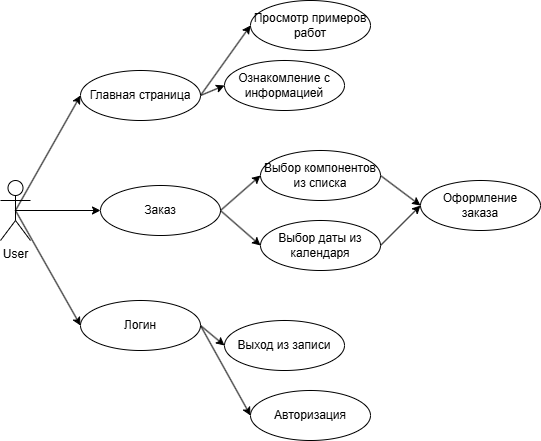
\includegraphics[width=0.8\linewidth]{userdp}
	\caption{Диаграмма прецедентов}
	\label{userdp:image}
\end{figure}
\clearpage
\begin{figure}[h]
	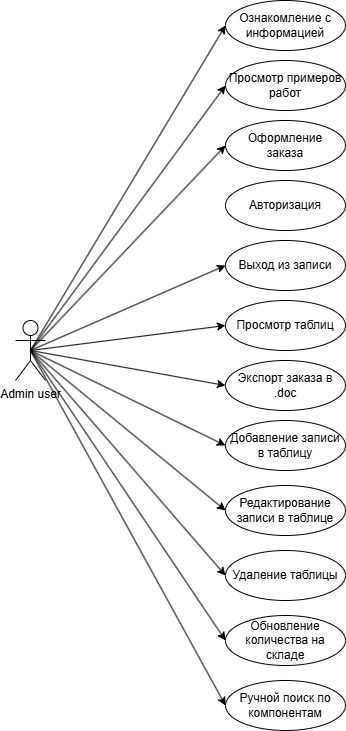
\includegraphics[width=0.7\linewidth]{aduserdp}
	\caption{Диаграмма прецедентов админа}
	\label{aduserdp:image}
\end{figure}
\clearpage

\subsubsection{Вариант использования «Ознакомление с информацией»}
Заинтересованные лица и их требования: пользователь желает узнать базовую информацию о Pc-Club, посмотреть на готовые сборки.
Предусловие: Открыт поисковик.
Постусловие: Пользователь заинтересован оформлением заказа у Pc-Club.
\begin{enumerate}
	\item Пользователь вводит адрес программно-информационной системы или ищет её по названию Pc-Club.
	\item Пользователь попадает на главную страницу сервиса.
	\item Пользователь ознакамливается с преимуществами.
	\item Пользователь смотрит примеры выполненных работ.
\end{enumerate}

\subsubsection{Вариант использования «Оформление заказа»}
Заинтересованные лица и их требования: Заинтересованный пользователь хочет быстро и удобно оформить заказ.
Предусловие: Открыта главная страница программно-информационной системы.
Постусловие: Был оформлен заказ и его запись отправилась в sql.
\begin{enumerate}
	\item Пользователь с помощью навигационной панели или кнопки "Начать сборку".
	\item Пользователь попадает на страницу оформления заказа.
	\item Пользователь вводит данные.
	\item Пользователь выбирает даты из календаря.
	\item Пользователь нажимает на компонент.
	\item Пользователь вводит название интересующего компонента/выбирает из представленного.
	\item Пользователь нажимает на кнопку "оформить заказ".
	\item Система проверяет введенные данные через validator.
	\item Система вычитает из имеющегося числа компонентов, задействованные.
	\item Система отправляет подготовленный sql запрос с предоставленными данными.
	\item Запись добавляется в sql и заказ принят к работе.
\end{enumerate}

\subsubsection{Вариант использования «Регистрация»}
Заинтересованные лица и их требования: Пользователь хочет зарегистрировать новую учетную запись.
Предусловие: Открыта главная страница программно-информационной системы.
Постусловие: Новая учетная запись сохранена в sql.
\begin{enumerate}
	\item Пользователь нажимает на кнопку "Войти".
	\item Пользователь вводит логин в поле.
	\item Пользователь вводит пароль в поле.
	\item Пользователь нажимает зарегистрироваться.
	\item Система подготовленным sql запросом отправляет логин, хэш пароля в базу данных.
	\item Система сохраняет данные в sql и к ним можно обратиться.
\end{enumerate}

\subsubsection{Вариант использования «Вход(в админ)»}
Заинтересованные лица и их требования: Пользователь хочет войти под учетной записью администратора.
Предусловие: Открыта главная страница программно-информационной системы.
Постусловие: Совершен вход в учетную запись администратора.
\begin{enumerate}
	\item Пользователь нажимает на кнопку "Войти" в навигации.
	\item Пользователь вводит логин администратора в поле.
	\item Пользователь вводит пароль администратора в поле.
	\item Пользователь нажимает войти.
	\item Система сравнивает логин и хэши паролей с имеющимися в sql.
	\item Система создает сессию, в нашем случае с правами администратора.
\end{enumerate}

\subsubsection{Вариант использования «Выход»}
Заинтересованные лица и их требования: Пользователь выйти из учетной записи.
Предусловие: Открыта главная страница программно-информационной системы, пользователь авторизован.
Постусловие: Пользователь выходит из учетной записи.
\begin{enumerate}
	\item Пользователь нажимает на кнопку "Выход" в навигации.
	\item Система убирает все данные авторизации из сессии.
\end{enumerate}

\subsubsection{Вариант использования «Просмотр таблиц»}
Заинтересованные лица и их требования: Пользователь хочет посмотреть содержимое таблиц.
Предусловие: Открыта главная страница программно-информационной системы, в текущей сессии есть права администратора.
Постусловие: Пользователь просматривает содержимое таблиц.
\begin{enumerate}
	\item Пользователь нажимает на кнопку "Админ панель" в навигации.
	\item Открывается страница панели администратора.
	\item Пользователь выбирает интересующий тип компонента.
	\item Система подгружает из sql интересующую таблицу.
	\item Система выводит интересующую таблицу.
	\item Пользователь просматривает содержимое таблицы.
\end{enumerate}

\subsubsection{Вариант использования «Просмотр таблиц»}
Заинтересованные лица и их требования: Пользователь хочет посмотреть содержимое таблиц.
Предусловие: Открыта главная страница программно-информационной системы, в текущей сессии есть права администратора.
Постусловие: Пользователь просматривает содержимое таблиц.
\begin{enumerate}
	\item Пользователь нажимает на кнопку "Админ панель" в навигации.
	\item Открывается страница панели администратора.
	\item Пользователь выбирает интересующий тип компонента.
	\item Система подгружает из sql интересующую таблицу.
	\item Система выводит интересующую таблицу.
	\item Пользователь просматривает содержимое таблицы.
\end{enumerate}

\subsubsection{Вариант использования «Редактирование таблиц»}
Заинтересованные лица и их требования: Пользователь хочет получить .doc файл с информацией по заказу.
Предусловие: Открыта админ панель.
Постусловие: Пользователь получает .doc файл.
\begin{enumerate}
	\item Пользователь выбирает таблицу заказы.
	\item Система подгружает из sql интересующую таблицу.
	\item Пользователь выбирает интересующую запись в таблице заказов.
	\item Пользователь нажимает на кнопку "Экспорт".
	\item Система формирует .doc файл с данными заказа.
	\item Система скачивает файл с информациями о сборке.
\end{enumerate}

\subsubsection{Вариант использования «Добавление в таблицу»}
Заинтересованные лица и их требования: Пользователь хочет добавить новую запись в таблицу.
Предусловие: Открыта админ панель.
Постусловие: Пользователь добавляет запись в таблицу.
\begin{enumerate}
	\item Пользователь выбирает интересующую таблицу.
	\item Система подгружает из sql интересующую таблицу.
	\item Система выводит таблицу.
	\item Пользователь нажимает на кнопку "+добавить" у нужной таблицы.
	\item Открывается страница для добавления нового элемента.
	\item Пользователь меняет требуемые данные в формах и нажимает "Добавить".
	\item Система проверяет введенные данные через validator.
	\item Система отправляет подготовленный sql запрос и сохраняет данные в sql.
\end{enumerate}

\subsubsection{Вариант использования «Удаление в таблице»}
Заинтересованные лица и их требования: Пользователь хочет удалить запись из таблицы.
Предусловие: Открыта админ панель.
Постусловие: Пользователь удаляет запись в таблице.
\begin{enumerate}
	\item Пользователь выбирает интересующую таблицу.
	\item Система подгружает из sql интересующую таблицу.
	\item Система выводит таблицу.
	\item Пользователь нажимает на кнопку с мусорным ведром у элемента.
	\item Браузер просит подтверждение действия.
	\item Пользователь нажимает "подтвердить".
	\item Система удаляет запись об элементе из sql.
\end{enumerate}

\subsubsection{Вариант использования «Обновления количества компонентов на складе»}
Заинтересованные лица и их требования: Пользователь хочет удалить запись из таблицы.
Предусловие: Открыта админ панель.
Постусловие: Пользователь обновляет количество компонента на складе.
\begin{enumerate}
	\item Пользователь нажимает на кнопку "склад" в навигации.
	\item Пользователь выбирает интересующую таблицу.
	\item Система подгружает из sql интересующую таблицу.
	\item Система выводит таблицу.
	\item Пользователь вводит новое количество компонента и нажимает "обновить".
	\item Система отправляет запрос в sql и сохраняет новое значение.
\end{enumerate}
\newpage
%-------------------------------------------------------------------------------
\subsection{Требования пользователя к интерфейсу веб-приложения}

Композиция шаблона программно-информационной системы представлена на рисунке ~\ref{indext:image}.

\begin{figure}[ht]
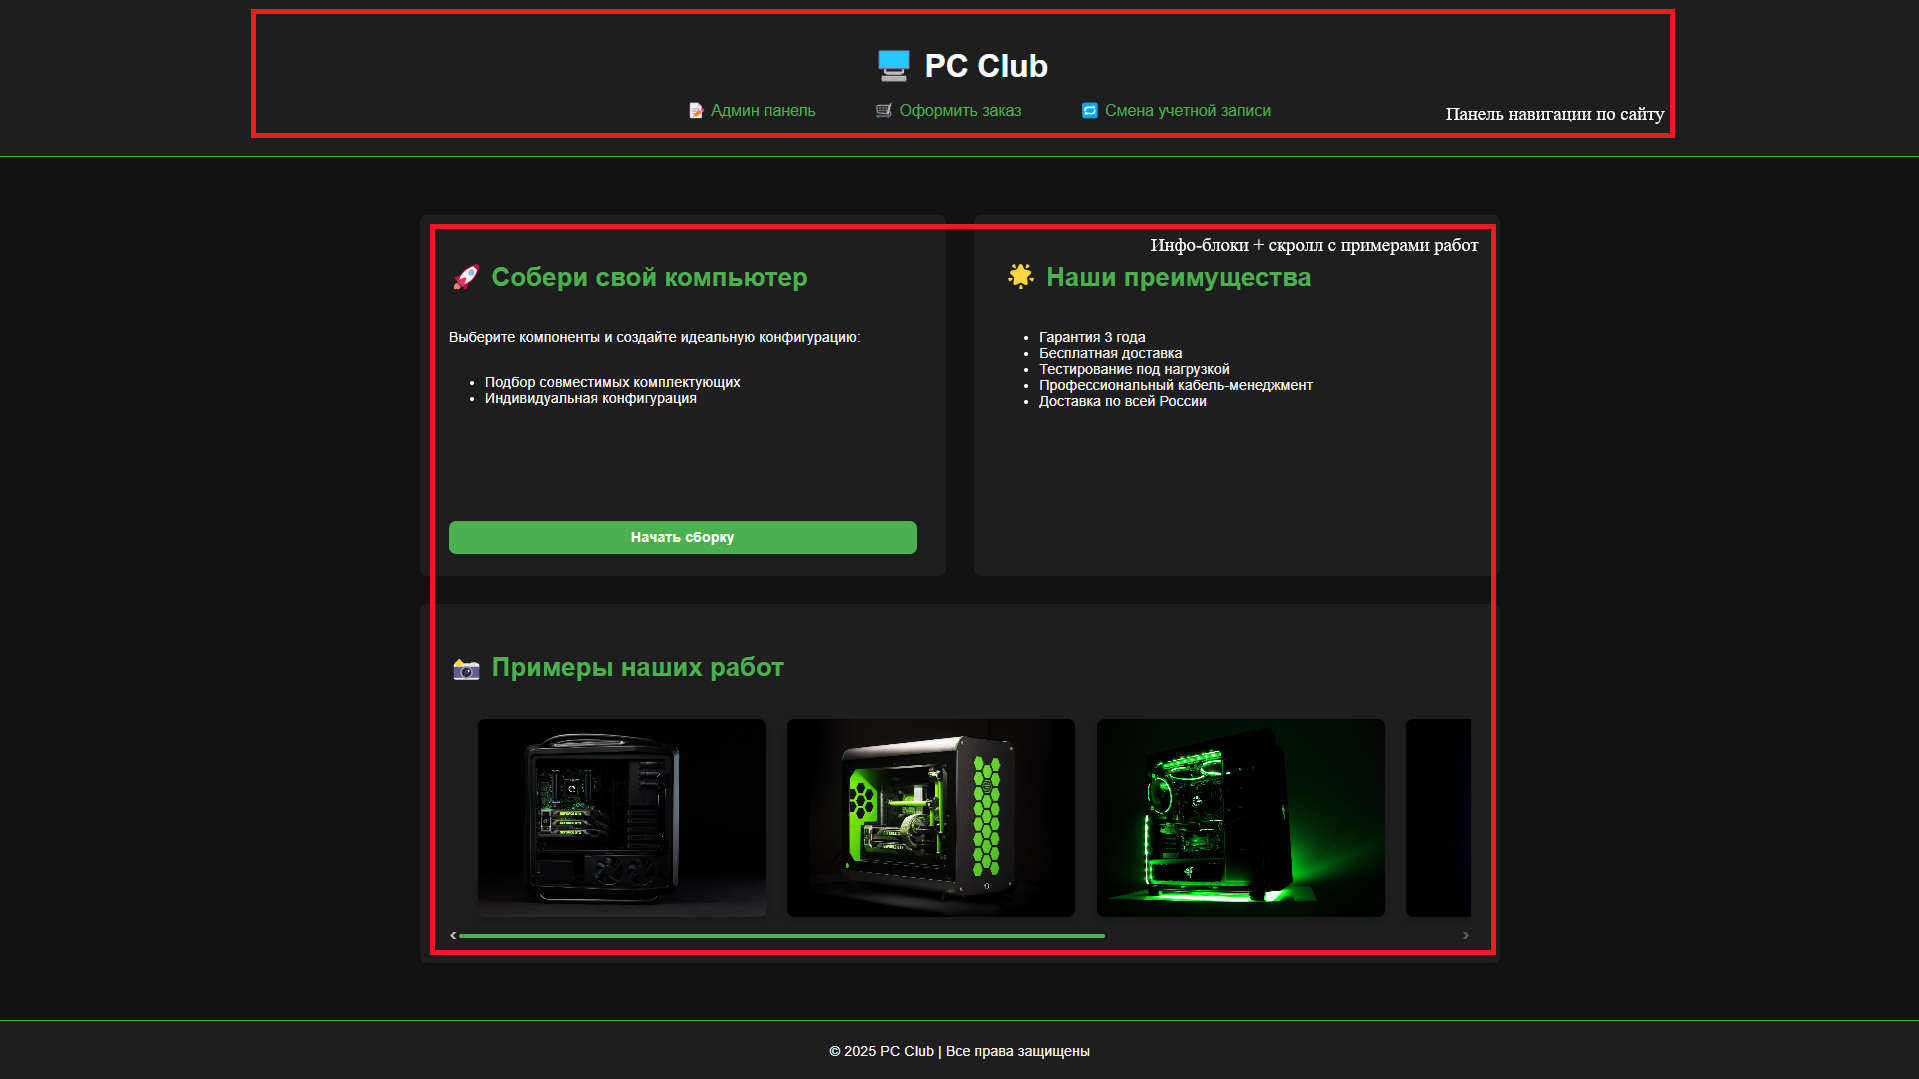
\includegraphics[width=1\linewidth]{indext}
\caption{Композиция шаблона программно-информационной системы}
\label{indext:image}
\end{figure}

\subsubsection{Гланая страница index}

Главная страница позволяет пользователю узнать основную информацию о деятельности сервис центра, посмотреть на существующие работы и должна заинтересовать его в заказе конкретно у Pc--Club. Главная страница, должна иметь элементы навигации для перемещения по программно-информационной системе и получения доступа к разному контенту, аналогично и на других страницах.

\subsubsection{Страница авторизации login}

На странице авторизации пользователь или сотрудник могут совершить вход в существующую учетную запись или создать новую. Важно, регистрировать учетную запись администратора запрещено, можно только редактировать через систему. На странице должны быть аналогично index панель навигации и все необходимые инструменты для авторизации.

\subsubsection{Страница заказы orderform}

На этой странице пользователь или сотрудник может оформить заказ в удобном интерфейсе, после оформления заказа тот отправляется в базу данных на хранение. Каждый компонент можно удобно выбрать из выпадающего списка с поиском, а даты выбирать в открывающемся календаре.

\subsubsection{Страница админ панели editcontent}

Доступ к этой странице может получить только пользователь с учетной записью администратора, здесь можно редактировать какие вообще компоненты доступны, добавлять новые или удалять, просматривать информацию о заказах и редактировать её. Здесь у нас расширенная панель навигации позволяющая открыть к прочим еще страницу "склад", о ней дальше.

\subsubsection{Страница админ панели stockmanagment}

Доступ к этой странице аналогично, только у администратора, тут также расширенная панель навигации с доступом ко всем вкладкам. На самой странице сотрудник может пополнить количество любого недостающего компонента.

\subsection{Нефункциональные требования к программной системе}

\subsubsection{Требования к безопасности}
Для безопасности хранимых данных пользователей требуется сохранять пароли в формате  хэш-кодов. Стабильность работы самой базы данных может кто-то попытаться нарушить с помощью sql-иньекции, защититься от этого можно используя подготовленные sql запросы и валидацию принимаемых данных с помощью регулярных выражений.
\subsubsection{Требования к программному обеспечению}
Для реализации проекта потребуются такие Яп. как:
\begin{itemize}
	\item Html - разметка и структура веб-страницы;
	\item Php - сценарии и взаимодействия;
	\item JavaScript - сложные функции и некоторая логика;
	\item CSS - внешний вид страниц и кастомизация элементов.		
\end{itemize}

Также для создания базы данных и работы с ней на этапе разработки используется xampp, включающий в себя MySql для базы данных и Apache для создания локального веб-сервера. 

Для работы на персональном компьютере потребуется:
\begin{itemize}
	\item операционная система: Windows (XP и выше), Mac OS X 10.4+, Linux;
	\item оперативная память: минимум 1 ГБ;
	\item веб-браузер: современные версии Chrome, Firefox, Edge и др.,поддерживающие EcmaScript 6;
	\item подключение к интернету: обязательно для работы с веб-приложениями.		
\end{itemize}

В свою очередь требования для удаленного сервера:
\begin{itemize}
	\item операционная система Linux (Ubuntu, CentOS, Debian) или Windows Server, Linux предпочтительнее;
	\item минимум 2–4 ГБ оперативной памяти;
	\item процессор 1.5 GHz и выше;
	\item объём дискового пространства от 10 ГБ и больше;
	\item стабильный, высокоскоростной интернет с публичным IP-адресом.		
\end{itemize}
\subsection{Требования к оформлению документации}

Разработка программной документации и программного изделия должна производиться согласно ГОСТ 19.102-77 и ГОСТ 34.601-90. Единая система программной документации.